\chapter{Hardware Development}

One of the cornerstones of our team's Concept of Operations for the SubT Challenge was modular autonomy. That is, we wanted to develop a series of modules which could be composed and rapidly reconfigured to suit the task at hand. The use of individual modules would also allow for components to be replaced or upgraded as necessary. For example, each of our ground robots had 4 drive modules, each consisting of a wheel, motor, gearbox, and a separate electronics module. The drive modules could be replaced or upgraded as necessary, such as in the case of a gearbox failing or the selection of different desired torque profiles. Similarly, we wanted to develop modular sensing and compute payloads which could be transferred across different robots, including in between ground and aerial robots, and which would be capable of performing all of the robot's high level autonomy functions.

Early indication that our approach should be feasible came as the result of using a prototype state estimation payload ("Blue Payload") similar to the Kaarta Traak \cite{kaarta_traak}. The payload was relatively small, self-contained, and could be easily transferred between robots (see Figure \ref{blue payload robots}). We simply had to mount the payload to the robot, apply power, and connect to the robot's internal network, and all of the payload's autonomy functions would be enabled. Overall, we found the Blue Payload quite simple to integrate, and wanted our future payloads to be similar in this regard. Inspired by the Blue Payload, and keeping the SubT Challenge requirements and timeline in mind, we came up with a list of some design goals and desired capabilities for our first payload ("Mk 0"), sorted by priority:

\begin{description}
	\item[Self-contained] All of the sensing and computation for the high level autonomy features should happen inside the payload itself. Ideally, the payload would only be supplied power and a network connection, just like the Blue Payload, and would output autonomy goals (such as waypoints) and information (such as robot state, maps, and artifact locations) to be relayed to the human supervisor at the base station.
	\item[Rapid Development] From the beginning of the competition (September 2018) to the first qualification deadline (December 2018), we had a little under 3 months to develop our first payload. This meant that, wherever possible, we should prefer designs that relied on existing expertise, such as the use of familiar components and sensors, and preferring in-house manufacturing capabilities with short lead times.
	\item[Environmentally Robust] We expected the field environments for the SubT competition to be somewhat hostile to the sensors. Specifically, we were told that "dust, fog, mist, water, and smoke are within scope" \cite{tunnel_rules}, and we wanted our payload to be reasonably protected against these elements, within reason. Additionally, the payload needed to be robust to the mechanical loading it would be subject to as a result of the rough terrain.
	\item[Weight Sensitivity] Similar to the Blue Payload, we wanted our new payload to be light enough to be carried by one of our aerial robots (as in Figure \ref{d1 blue payload}), or a smaller ground robot (as in Figure \ref{joeybot blue payload}) in addition to larger robots (as in Figure \ref{r1 blue payload}).
	\item[Low Cost] While there aren't specific restrictions on the maximum cost of our robot, DARPA was interested in identifying cost effective solutions for the SubT Challenge. Minimizing cost is also useful as a design goal as we intended to build multiple copies of the payload for our various robots, as well as to have spares.
\end{description}

\begin{figure}
	\centering
	\begin{subfigure}{0.3\textwidth}
		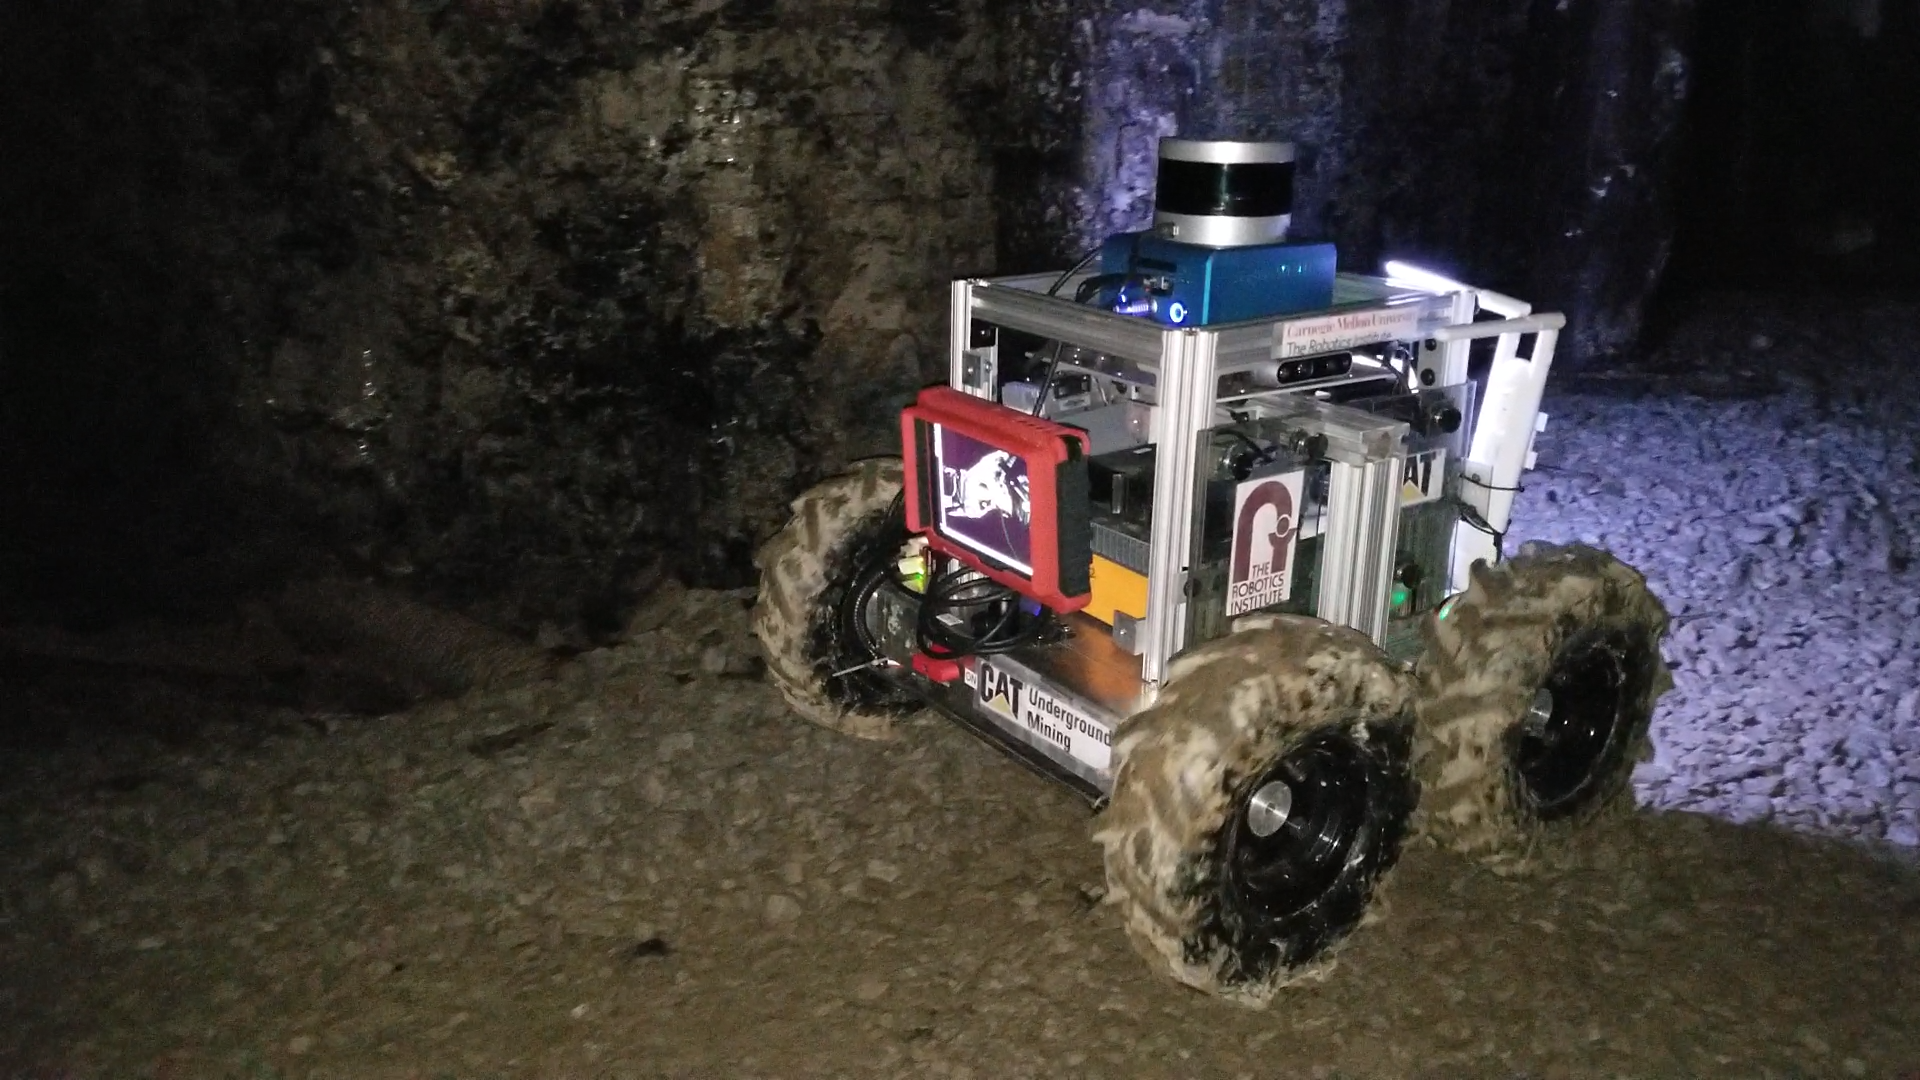
\includegraphics[width=\textwidth]{blue_payload_joeybot.png}
		\caption{Joeybot with Blue Payload}
		\label{joeybot blue payload}
	\end{subfigure}		
	\hfill
	\begin{subfigure}{0.3\textwidth}
		\includegraphics[width=\textwidth]{r1_with_blue_payload.jpg}
		\caption{R1 with Blue Payload}
		\label{r1 blue payload}		
	\end{subfigure}
	\hfill
	\begin{subfigure}{0.3\textwidth}
		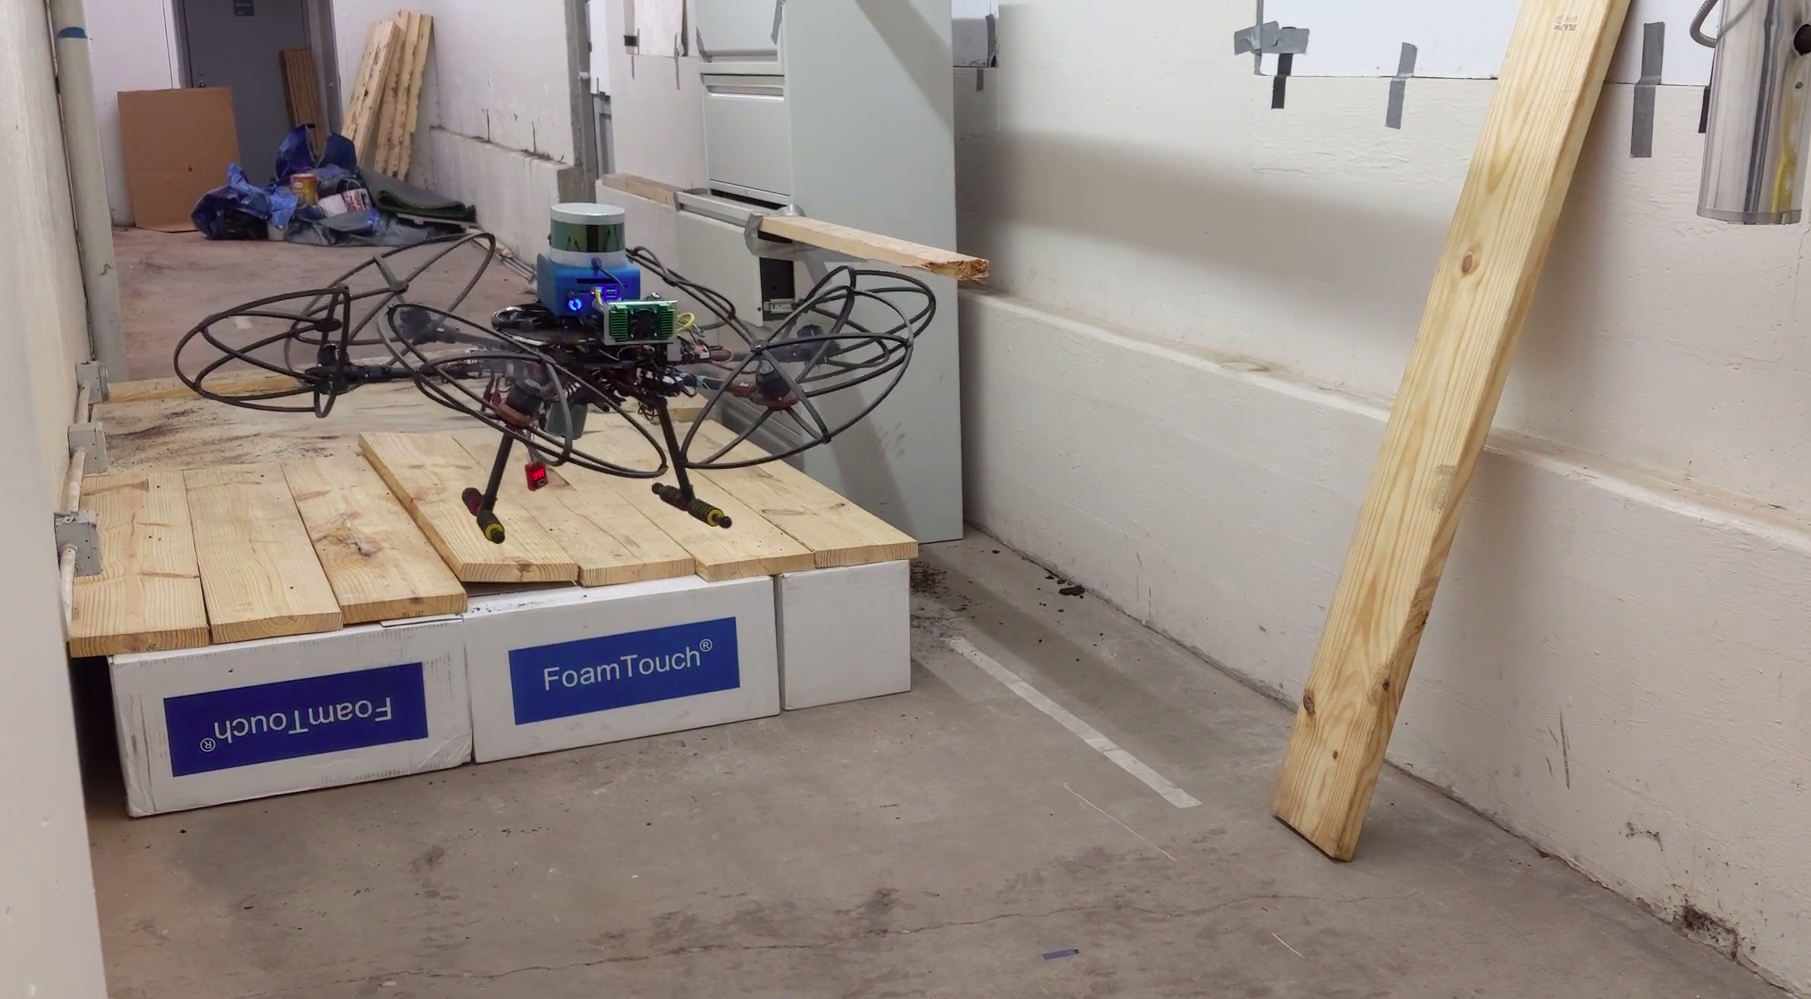
\includegraphics[width=\textwidth]{drone_with_blue_payload.png}
		\caption{D1 with Blue Payload}
		\label{d1 blue payload}
	\end{subfigure}	
	\caption{Robots with initial modular payload ("Blue Payload")}
	\label{blue payload robots}
\end{figure}

\section{Mk. 0 Component Selection}

\subsection{Computers}

In order to select the computer(s) to be used inside Mk. 0, it was important for us to figure out the tasks that the payload would need to perform. While we wouldn't be able to know exactly how many resources each of the tasks would consume, prior experience could help us determine some rough approximations. The main tasks for the payload would be the following:

\begin{enumerate}
	\item State estimation
	\item Path planning and navigation
	\item Object detection and localization
\end{enumerate}

For state estimation, we knew that we would be using LOAM \cite{zhang2014loam}, which was written by Ji Zhang (one of our team members), and is the current state of the art for SLAM. We knew that LOAM ran well on the Blue Payload, which uses an Intel NUC with an Intel Core i7 processor internally. The path planning and navigation stack was being actively developed and ran on the second computer on Joeybot (see Figure \ref{joeybot blue payload}), which was a mid-range industrial-grade PC from Logic Supply. Though the Logic Supply computer was also using an Intel Core i7 processor, the processor itself was underclocked to reduce heat output. Profiling indicated that it should be possible to run the path planning and navigation stack on the NUC being used to run LOAM, especially given the underclocked processor in the Logic Supply computer. This factor, along with various team members' familiarity with the NUC family of products, marked the Intel NUC as a strong contender for use in our payload. Specifically, we considered the NUC8i7BEB, which the best (with regards to CPU) available NUC board at the time.

Working under the assumption that we'd use an Intel NUC inside the payload, the question of running the object detection and localization stack still remained. While it wasn't yet clear what our object detection strategy would be, the use of convolutional neural networks in advancing the state of the art for object detection suggested that they would be a component of our approach. To efficiently run convolutional neural networks, a few hardware platforms were considered. We attempted to find a platform which we thought could run multiple neural networks in parallel, at relatively high frequencies (10+ Hz). We considered the following options:

\begin{enumerate}
	\item Intel Movidius Neural Compute Stick
	\item NUC8i7BEB integrated GPU (Intel Iris Plus Graphics 655)
	\item Nvidia Jetson TX2
	\item Nvidia Jetson AGX Xavier
\end{enumerate}

Of the available options, the Nvidia Jetson AGX Xavier ("Xavier") offered the highest inference performance due to its many CUDA cores, as well as its specialized Tensor Cores and Deep Learning Accelerators. Combined, the Xavier was capable of performing more than an order of magnitude more FLOPS than the other platforms. As we were unsure of the exact requirements of our object detection system at the time, we chose to overprovision, and thus the available FLOPS became the deciding factor. The Xavier emerged as the clear winner for our GPU selection inside the Mk. 0 payload. At this stage, it was also decided to commit to using the NUC8i7BEB inside Mk. 0. In an attempt to simplify the system, we briefly considered attempting to run the entire autonomy stack on a single Xavier, rather than split between a NUC and an Xavier. However, we felt that the slower ARM cores on the Xavier would not be able to handle the combined autonomy stack, and thus decided to continue using both computers inside the Mk. 0 payload. The NUC would handle the state estimation and path planning and navigation tasks while all object detection and localization tasks would run on the Xavier.

After the completion of the Mk. 0 payload, we performed some experiments to see if our earlier hypothesis about the Xavier being unable to handle the entire autonomy stack was correct. Profiling of the NUC revealed that LOAM was one of the heaviest processes, consuming nearly 100\% of a single core in some circumstances, and smaller portions of other cores. Thus, we decided to attempt to run LOAM on the Xavier first. For our benchmarking, we set up an Xavier Developer Kit in MAX-N mode after having disabled the frequency governors with the provided jetson\_clocks.sh script. This mode enables all of the processors in the Xavier, and pins them at their highest frequency. We attempted to run LOAM on pre-recorded data in a few different configurations, varying a parameter to adjust downsampling of the input point clouds to reduce the scan alignment cost. Figure \ref{loam_xavier} shows a visualization of the results.

\begin{figure}
	\centering
	\begin{subfigure}{0.3\textwidth}
		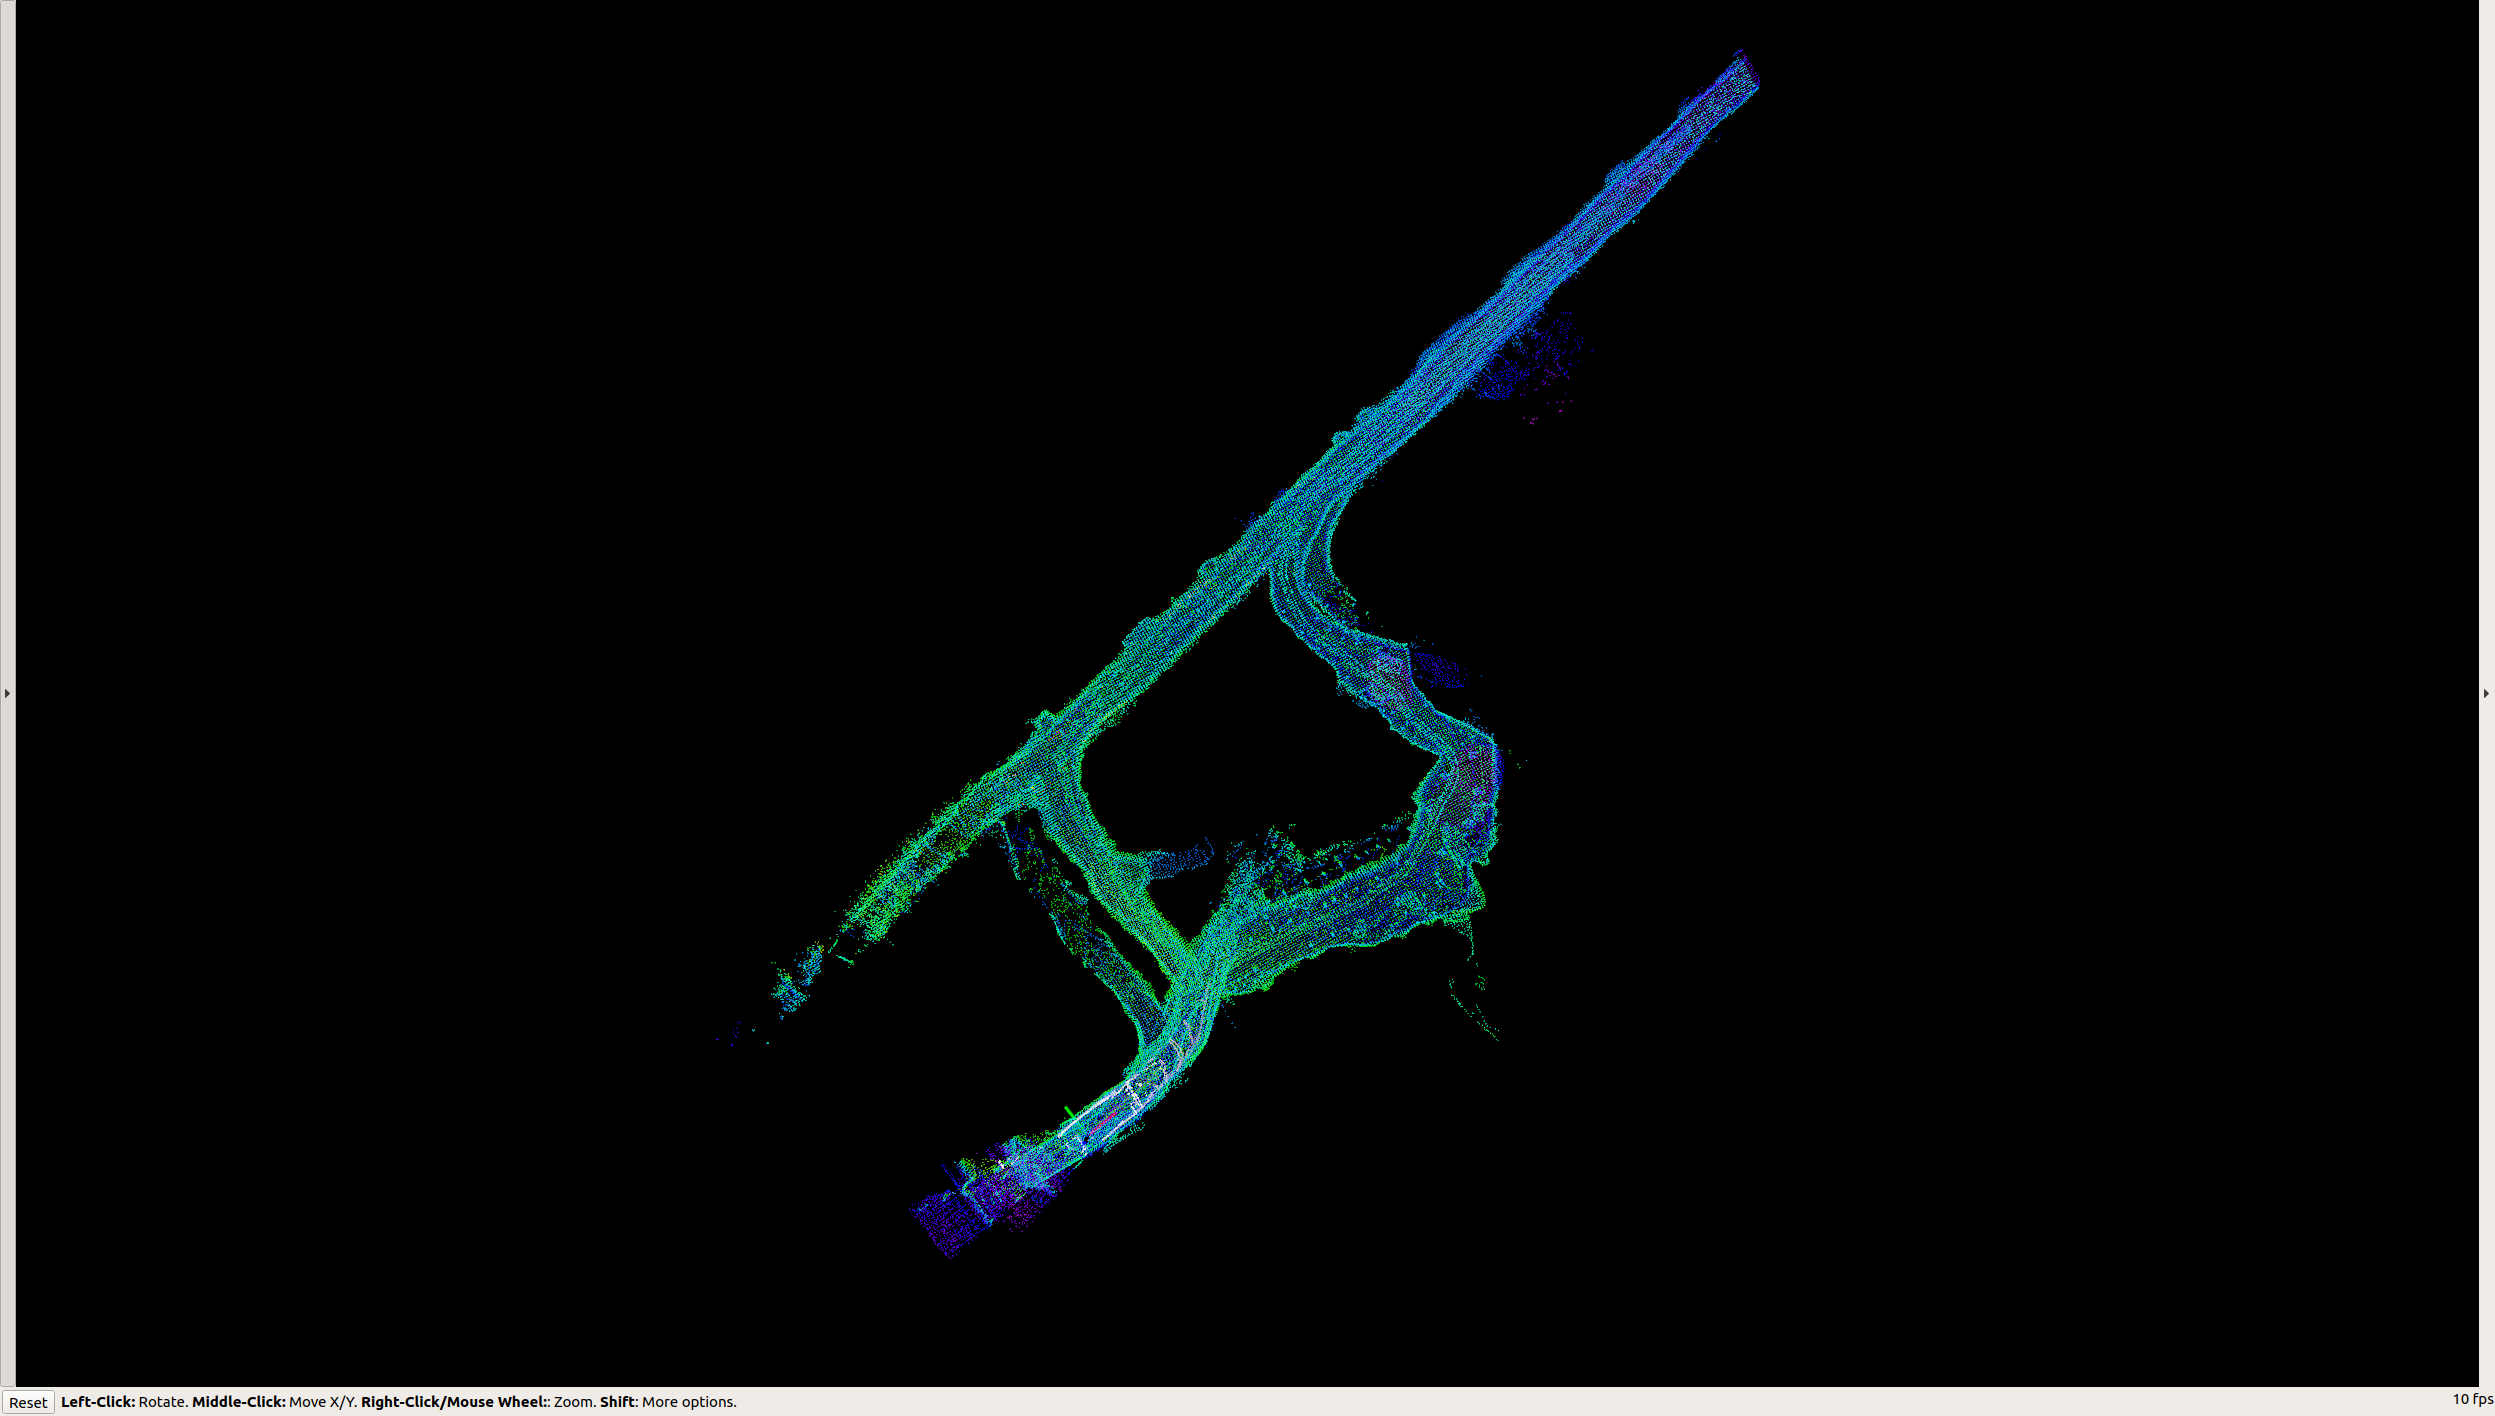
\includegraphics[width=\textwidth]{tour_ed_mine_1-00.png}
		\caption{100\% Point Cloud Scaling}
		\label{loam_xavier_100}
	\end{subfigure}		
	\hfill
	\begin{subfigure}{0.3\textwidth}
		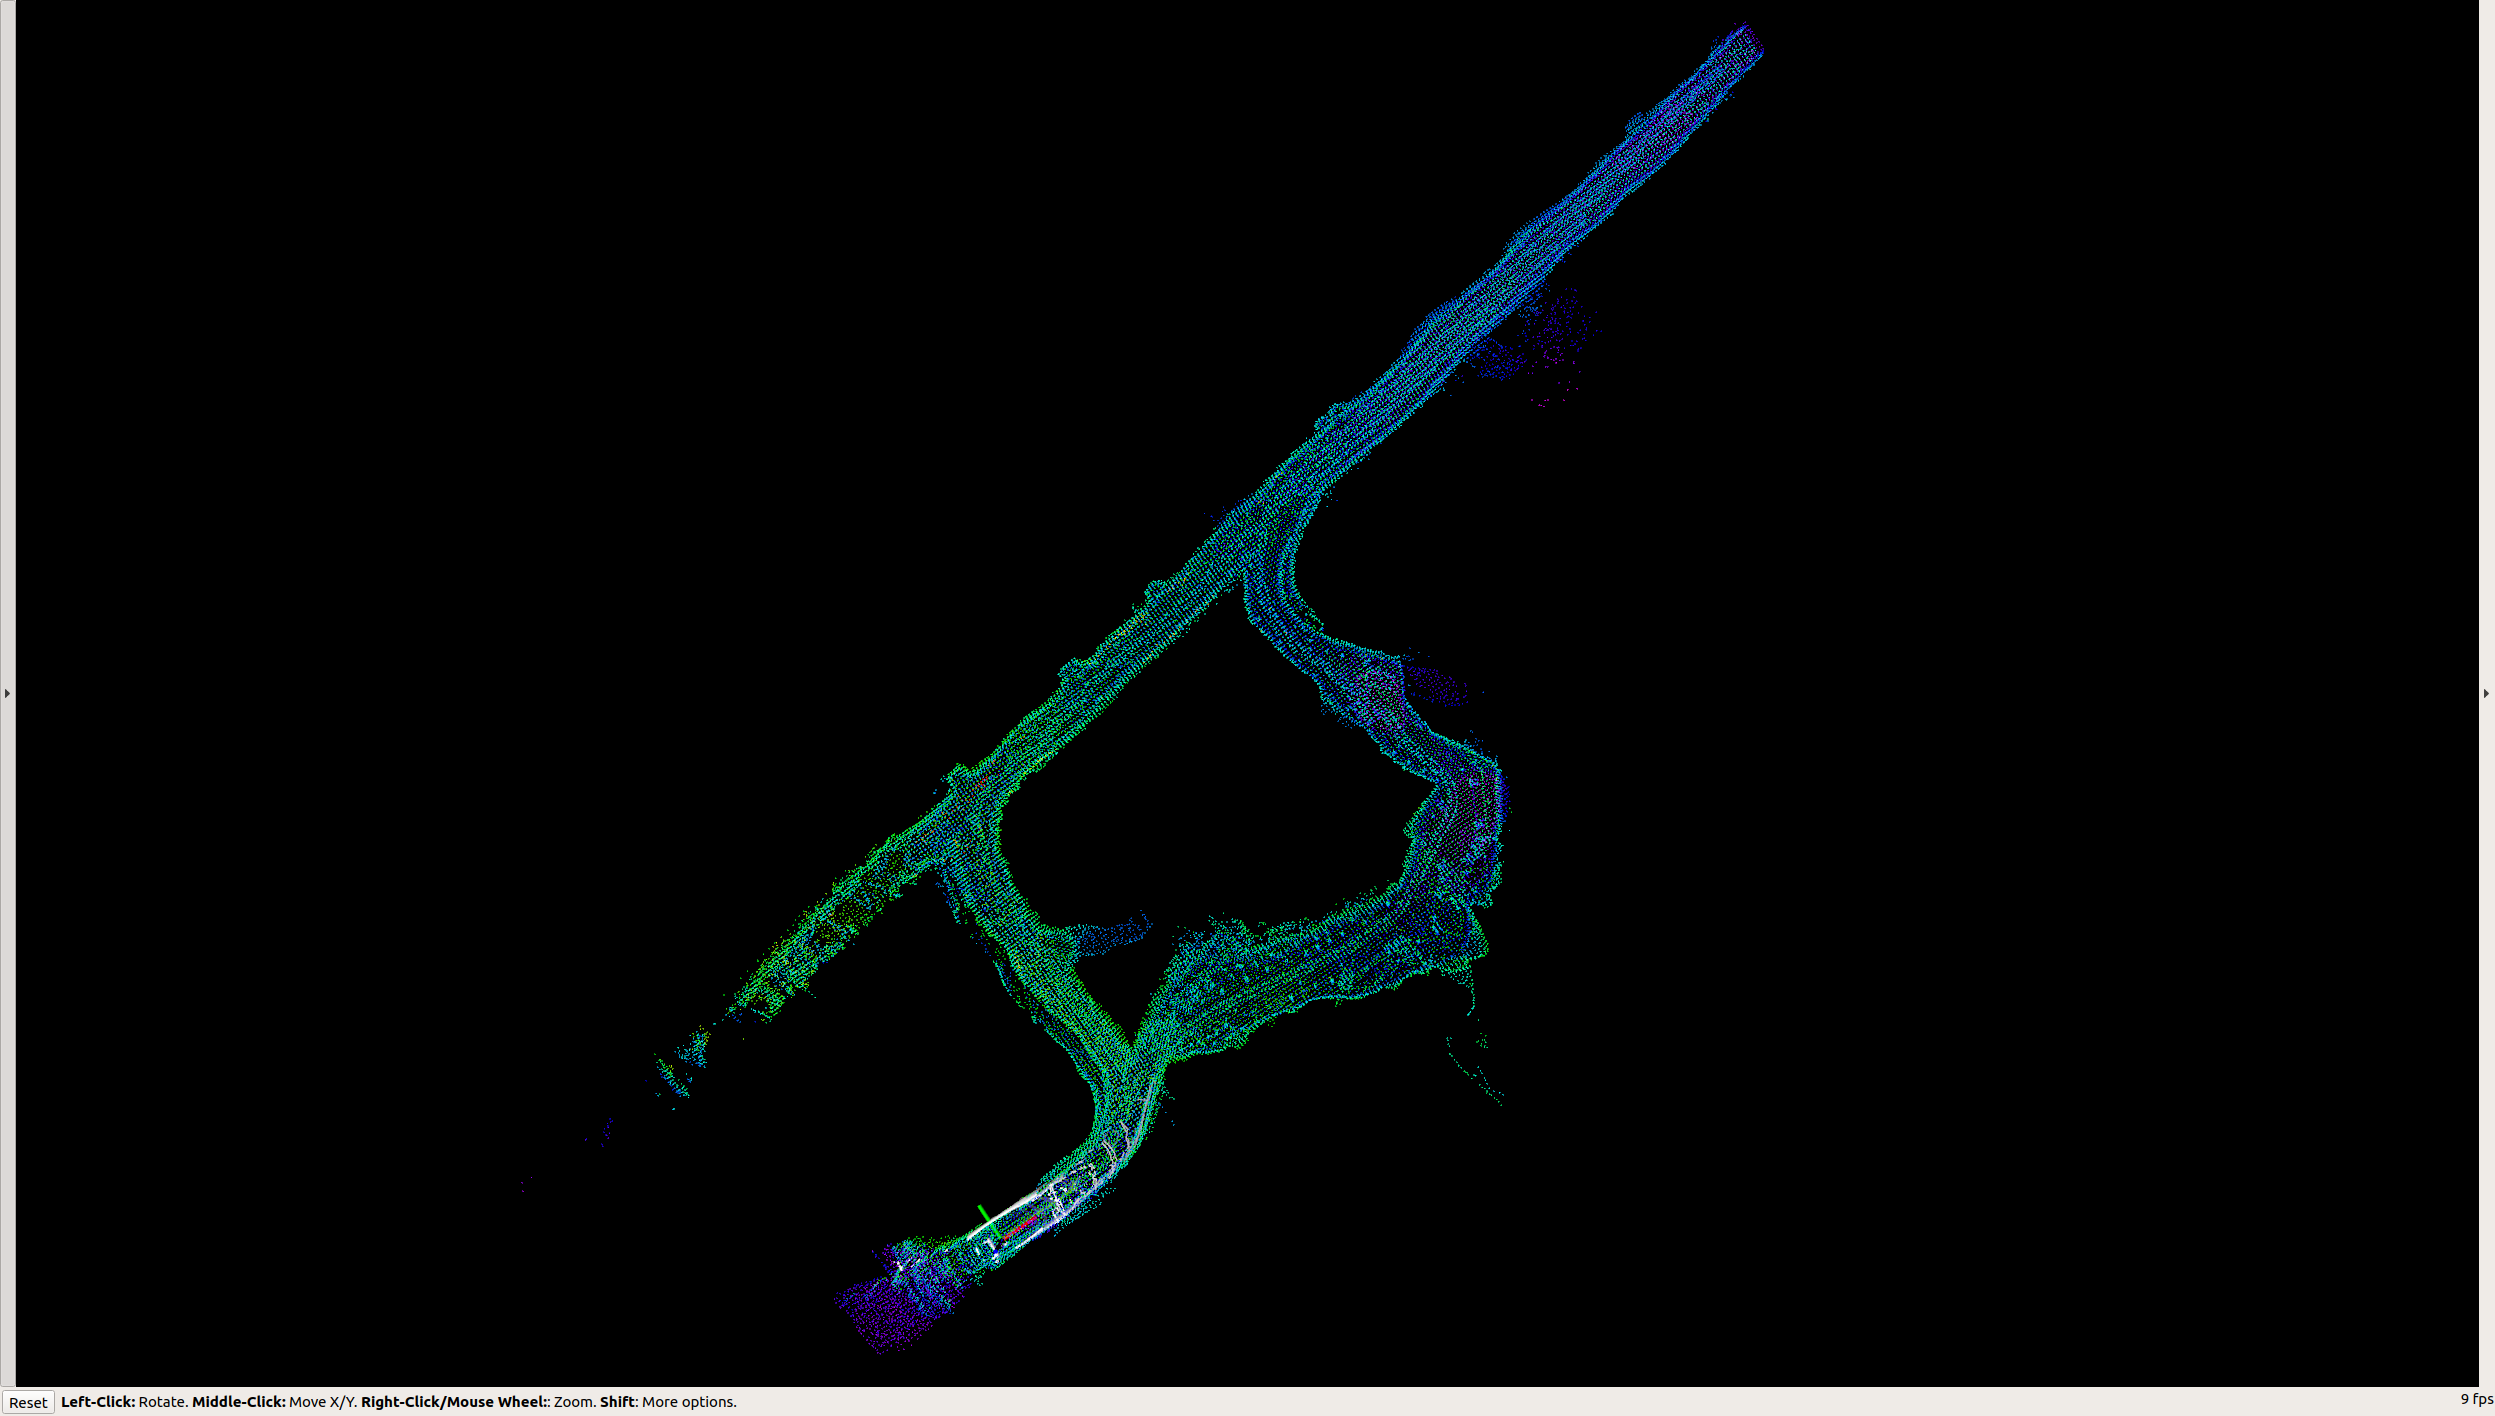
\includegraphics[width=\textwidth]{tour_ed_mine_1-00_1-25s.png}
		\caption{75\% Point Cloud Scaling}
		\label{loam_xavier_75}		
	\end{subfigure}
	\hfill
	\begin{subfigure}{0.3\textwidth}
		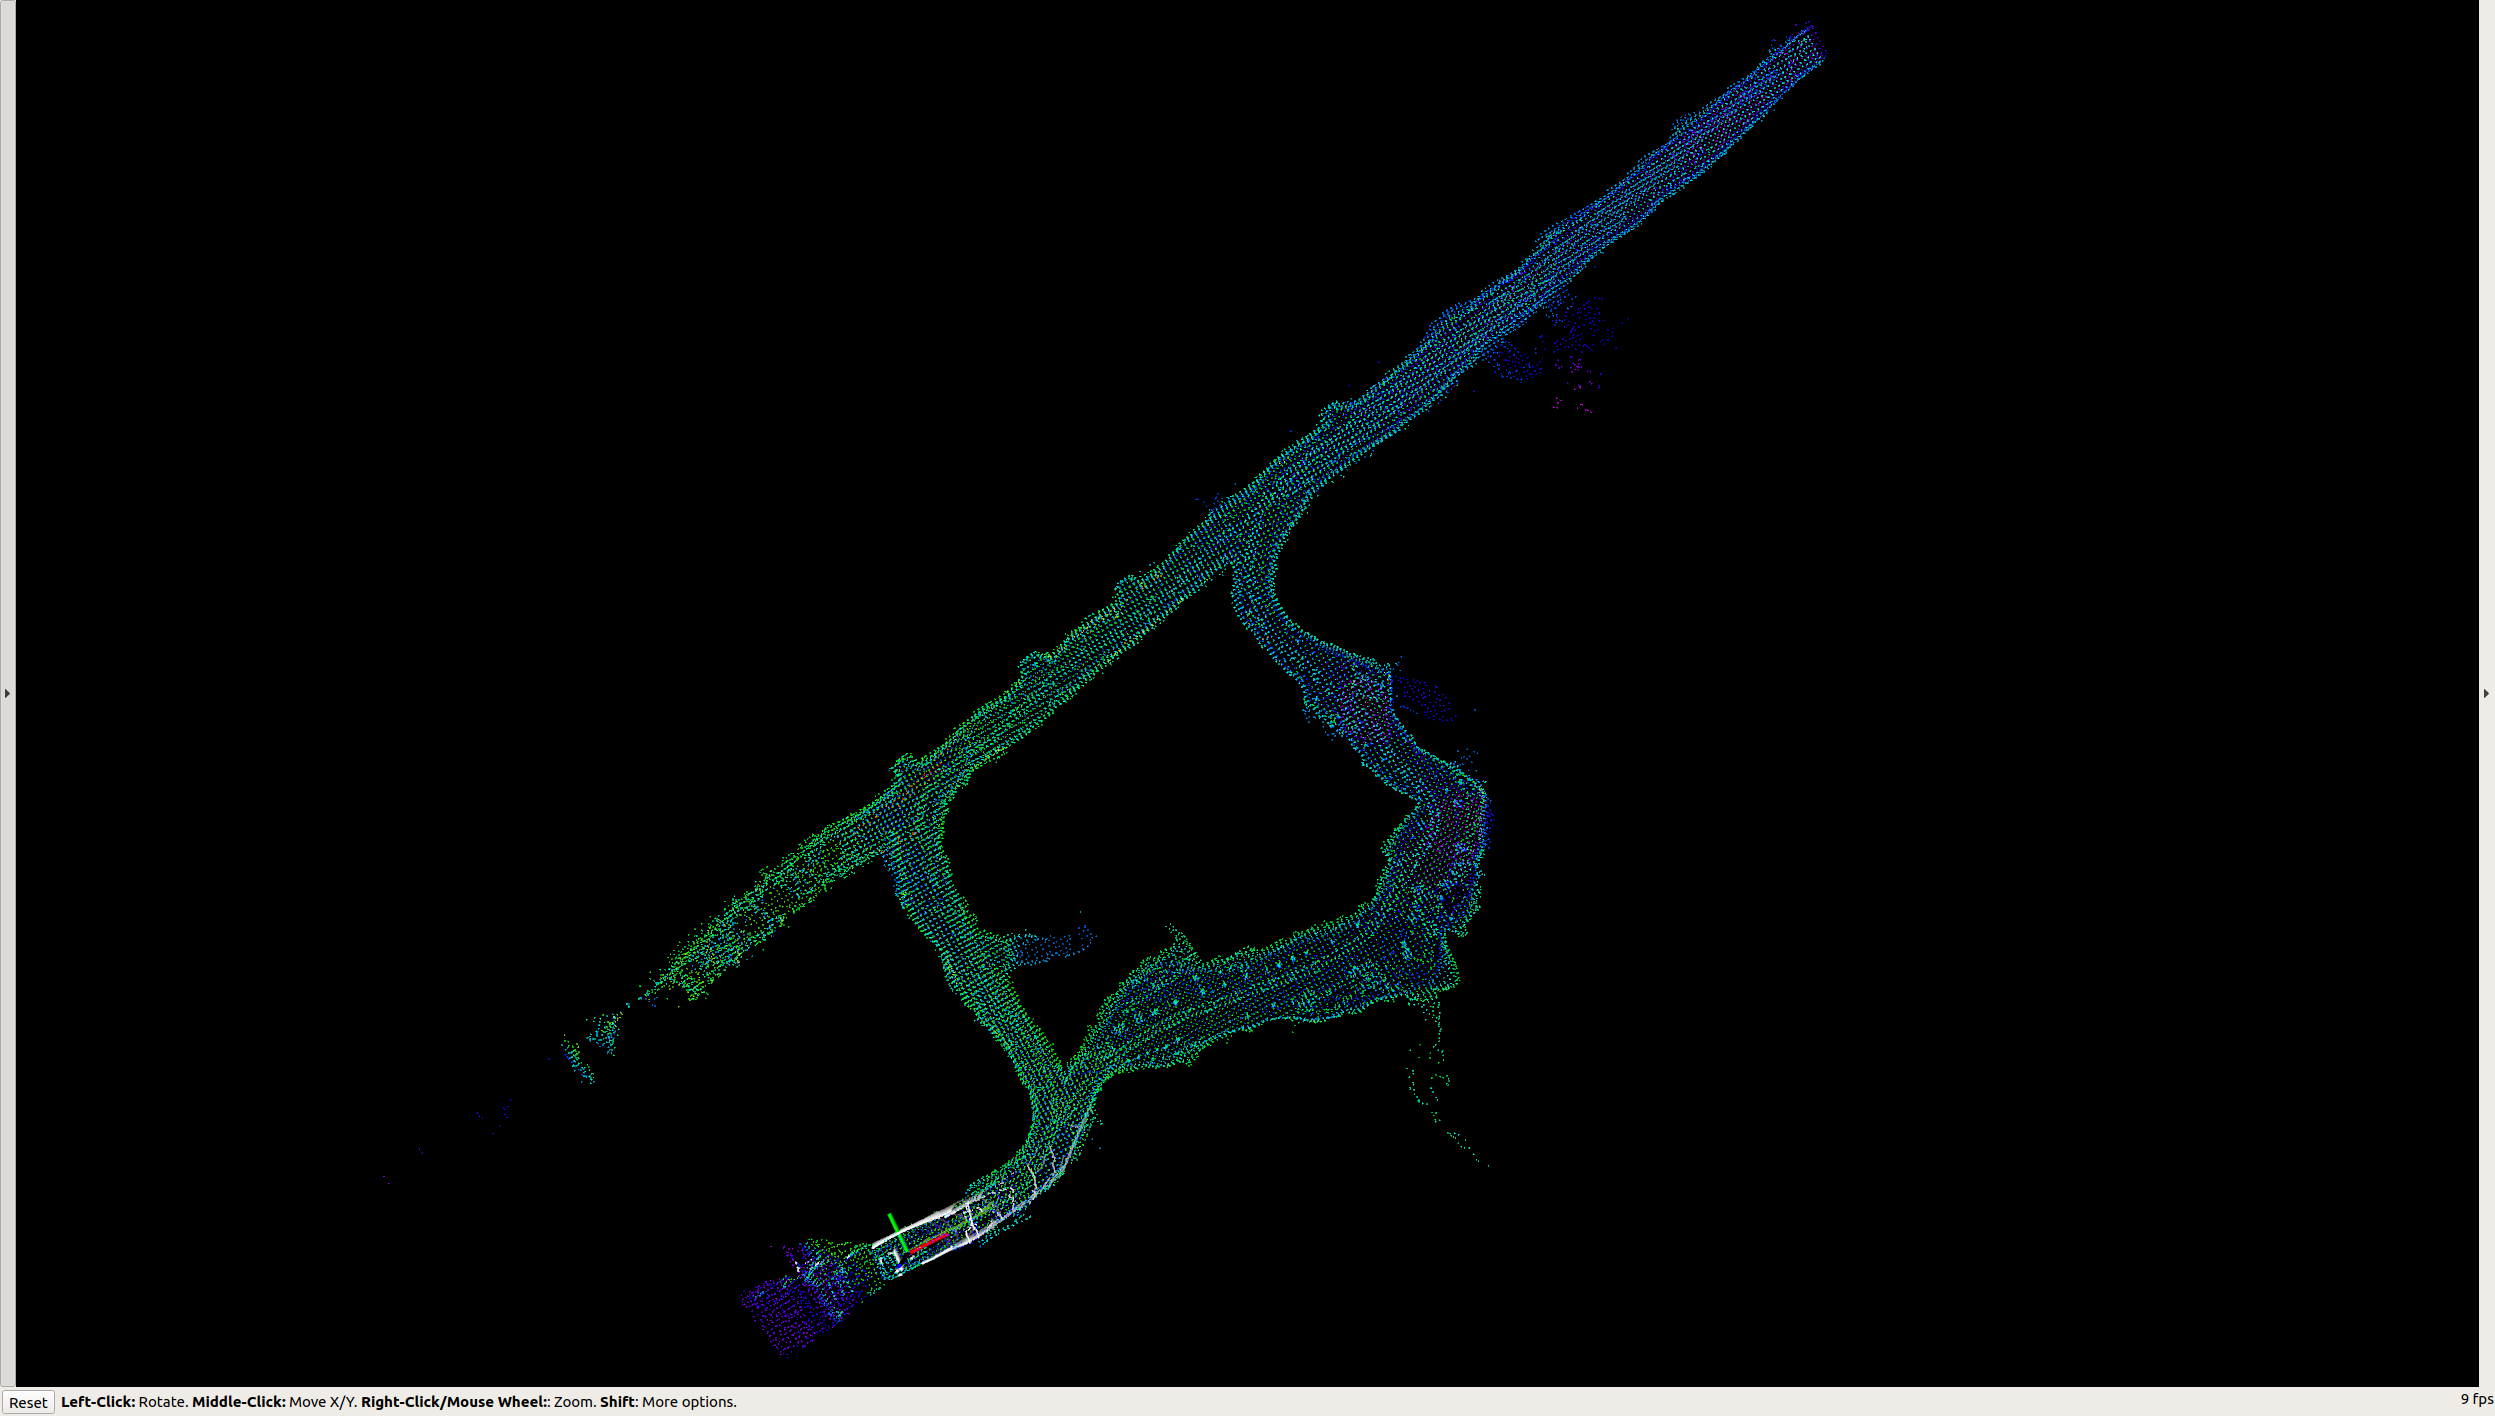
\includegraphics[width=\textwidth]{tour_ed_mine_1-00_1-50s.png}
		\caption{50\% Point Cloud Scaling}
		\label{loam_xavier_50}
	\end{subfigure}	
	\caption[Visualization of LOAM running on an Xavier]{Visualization of LOAM running on an Xavier with different downsampling parameters, using pre-recorded data collected at the Tour-Ed Mine in Tarentum, PA.}
	\label{loam_xavier}
\end{figure}

In Figure \ref{loam_xavier_100}, the same configuration as the NUC on Mk. 0 was used. Severe misalignment is visible - the lower tunnel does not align correctly, and a secondary "ghost" tunnel is created. In Figure \ref{loam_xavier_75}, 75\% of the laser scanner's points are kept. This does result in better alignment, though the images of two tunnels are still clearly visible in the figure. Finally, in Figure \ref{loam_xavier_50}, only 50\% of the laser scanner's points are kept. In this environment, the point cloud alignment is successful, suggesting that the state estimate did not drift significantly. However, the requisite 50\% downsampling was deemed to be too significant, as it presented a high risk of misalignment under harsh motions or in feature-bare environments due to the low density of points. This experiment confirmed our initial hypothesis that, without significant optimization, our current autonomy stack would be unable to run on a single Xavier.

\subsection{Sensors}

The first set of sensors selected for Mk. 0 were those necessary for state estimation. We selected exactly the same IMU and LIDAR (Velodyne VLP-16 Puck) as were used on the Blue Payload since LOAM was already proven to work with them. We then attempted to determine which sensors we would need to be able to identify all of the artifacts in the challenge. At this point in the competition, DARPA had not released a specific list of artifacts that would be used in the challenge, only general categories \cite{tunnel_rules}. We created a list of the types of sensors which we felt we could integrate into Mk. 0 in the short time available, and estimated the usefulness of each category of sensor in detecting artifacts from each category. A summary is presented in Table \ref{sensor_utility_categories}. The values were decided as follows:

\begin{itemize}
	\item High -- Artifacts of this category are expected to produce extreme sensor responses and be easy to distinguish.
	\item Medium -- Artifacts of this category are expected to be found with moderate difficulty in sensor data.
	\item Low -- Artifacts of this category are expected to be difficult or expensive to separate from sensor noise, perhaps due to a low response, or anticipated interference.
	\item None -- Artifacts of this category are expected to effect no response in sensors of this category.
\end{itemize}

% TODO(vasua): Do I need to add more information about how I came up with this table?

% https://www.tablesgenerator.com/#
\begin{table}[]
	\centering
	\resizebox{\textwidth}{!}{%
		\begin{tabular}{lccccccc}
			\hline
			& \textbf{\begin{tabular}[c]{@{}c@{}}RGB\\ Camera\end{tabular}} & \textbf{\begin{tabular}[c]{@{}c@{}}Thermal\\ Camera\end{tabular}} & \textbf{\begin{tabular}[c]{@{}c@{}}Depth\\ Camera\end{tabular}} & \textbf{LIDAR} & \textbf{Microphone(s)} & \textbf{\begin{tabular}[c]{@{}c@{}}Wifi / Bluetooth\\ Scanning\end{tabular}} & \multicolumn{1}{l}{\textbf{Gas Sensor}} \\ \hline
			\textbf{Survivors}                  & High                                                          & High                                                              & High                                                            & Medium         & Low                    & None                                                                         & None                                    \\ \hline
			\textbf{Ingress / Egress Points}    & Medium                                                        & Low                                                               & High                                                            & Medium         & Low                    & None                                                                         & Low                                     \\ \hline
			\textbf{Electric Pumps}             & High                                                          & High                                                              & Low                                                             & Medium         & Medium                 & None                                                                         & None                                    \\ \hline
			\textbf{Backpacks}                  & High                                                          & None                                                              & Low                                                             & Low            & None                   & None                                                                         & None                                    \\ \hline
			\textbf{Valves}                     & High                                                          & None                                                              & Low                                                             & None           & None                   & None                                                                         & None                                    \\ \hline
			\textbf{Radios / Cell Phones}       & Low                                                           & Medium                                                            & Low                                                             & None           & Medium                 & High                                                                         & None                                    \\ \hline
			\textbf{Tools / Fire Extinguishers} & High                                                          & None                                                              & Low                                                             & None           & None                   & None                                                                         & None                                    \\ \hline
			\textbf{Power Sources}              & Medium                                                        & High                                                              & Medium                                                          & Medium         & None                   & None                                                                         & None                                    \\ \hline
			\textbf{Oxygen Level}               & None                                                          & None                                                              & None                                                            & None           & None                   & None                                                                         & High                                    \\ \hline
			\textbf{Gas Leaks}                  & None                                                          & Medium                                                            & None                                                            & None           & Medium                 & None                                                                         & High                                    \\ \hline
		\end{tabular}%
	}
	\caption{Speculated utility of various sensor categories for DARPA provided artifact categories}
	\label{sensor_utility_categories}
\end{table}

Table \ref{sensor_utility_categories} indicates that while there is some redundancy across sensing categories in their speculated ability to detect various artifact categories, most of the sensor types have at least one artifact category that they alone would be highly likely to detect. For example, Wifi / Bluetooth Scanning is the only sensing category rated as "High" utility in detecting Radios / Cell Phones. Based on this table, Mk. 0 should contain at least some sort of RGB camera, thermal camera, depth camera, wifi / bluetooth scanner, and gas sensor in order to have a high chance of detecting each of the possible artifact categories. A LIDAR isn't required for object detection, but will necessarily be included for state estimation as described above. The microphone isn't strictly necessary, so we aimed to include it in the payload if it would be simple to do, but otherwise devote little attention to it. With our list of sensor types decided, we began experimenting with various products to identify specific models destined for inclusion in Mk. 0.

\begin{description}
	\item[RGB Camera] Having the highest overall utility across sensor categories, the RGB camera was the first sensor we aimed to select. The first selection criteria for the camera was the interface type. Three possibilities were considered -  CSI, Ethernet, and USB. CSI, capable of offering very high data rates with low latency, was the preferred interface. However, hardware and driver support for CSI cameras for the Xavier was still developing at this time, eliminating this option. Ethernet was considered for ease of integration. However, the larger size of Ethernet cameras and connectors, as well as the lower available bandwidth for multiple cameras forced us to eliminate this option as well. We were left with USB as our selection for camera interface. USB 3.0 offered the data rates we would need to use multiple cameras, but had the potential to suffer from high latency due to multiple levels of hardware and software buffering.
	
	With our choice of interface made, we considered two types of cameras for use in the Mk. 0 payload. The first was the UI-3241LE-C-HQ by IDS Imaging, a bare camera board that other members of our lab had successfully used on previous projects. The second was the Intel RealSense D435, selected for its inclusion of a stereo depth pair in a small form factor. When comparing the two cameras, in addition to the overall payload goals, there were a few camera-specific criteria we used when comparing the various cameras:
	
	\begin{enumerate}
		\item Low light performance - We expected the subterranean environments to dimly lit in general, and occasionally be completely dark. A camera with lower image noise in dark environments was preferred.
		\item Synchronization ability - Given the expected utility of the RGB cameras, as well as for redundancy, we anticipated using multiple cameras on Mk. 0. A hardware synchronization mechanism between the cameras and other payload sensors (e.g. LIDAR) would help increase the accuracy of various software algorithms.
		\item Shutter type - A global shutter was preferred due to the increased image quality under harsh camera motions, which was expected as a result of rough terrain.
	\end{enumerate}
	
	% TODO(vasua):  Provide additional images in the appendix, maybe? Not sure how necessary they are.
	To evaluate low light performance, we used the provided ROS drivers to capture images from both cameras at their native / recommended resolutions (1280 x 1024 for the UI camera, and 848 x 480 for the RealSense) across a range of manually selected exposure and gain values with the camera framerates set to 30 fps. The images shown in Figure \ref{camera_comparison} contain images of the same scene from both cameras with 33 ms exposure time and the minimum and maximum gains supported by the drivers. Additionally, images of a similar scene were captured with autoexposure enabled in each camera.
	
	\begin{figure}
		\centering
		\begin{subfigure}{0.3\textwidth}
			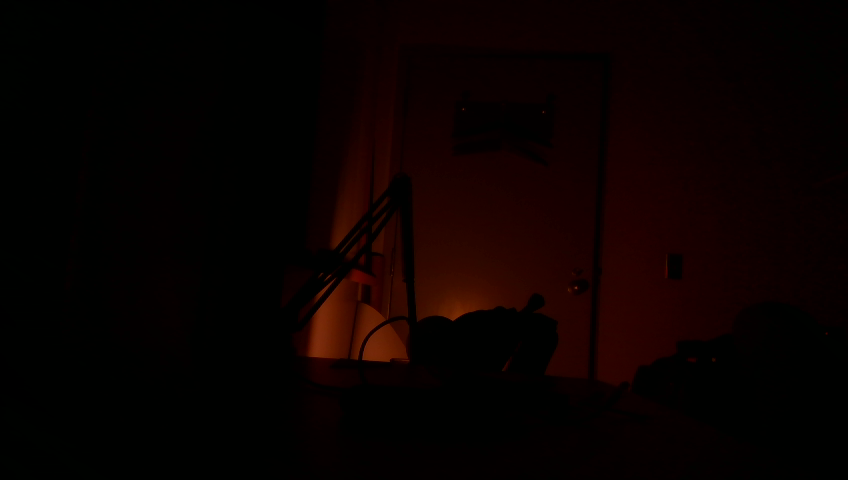
\includegraphics[width=\textwidth]{rs_img_33_ms_016.png}
			\caption{RealSense 33 ms exposure, minimum gain}
			\label{rs_img_33_ms_016}
		\end{subfigure}		
		\hfill
		\begin{subfigure}{0.3\textwidth}
			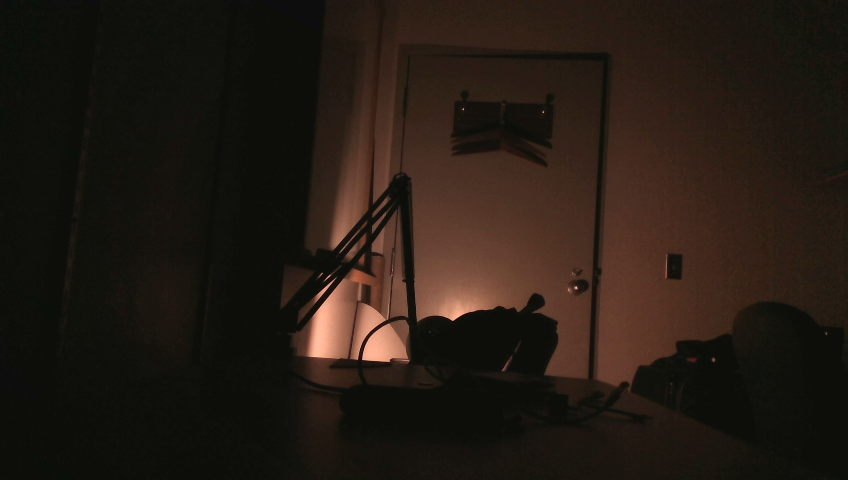
\includegraphics[width=\textwidth]{rs_img_33_ms_128.png}
			\caption{RealSense 33 ms exposure, maximum gain}
			\label{rs_img_33_ms_128}		
		\end{subfigure}
		\hfill
		\begin{subfigure}{0.3\textwidth}
			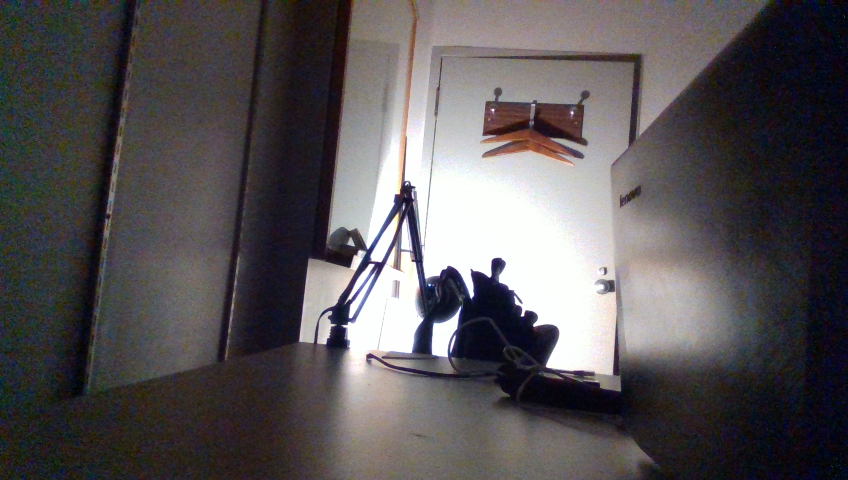
\includegraphics[width=\textwidth]{auto_realsense_2.png}
			\caption{RealSense automatic exposure, automatic gain}
			\label{auto_realsense_2}
		\end{subfigure}
		\\
		\begin{subfigure}{0.3\textwidth}
			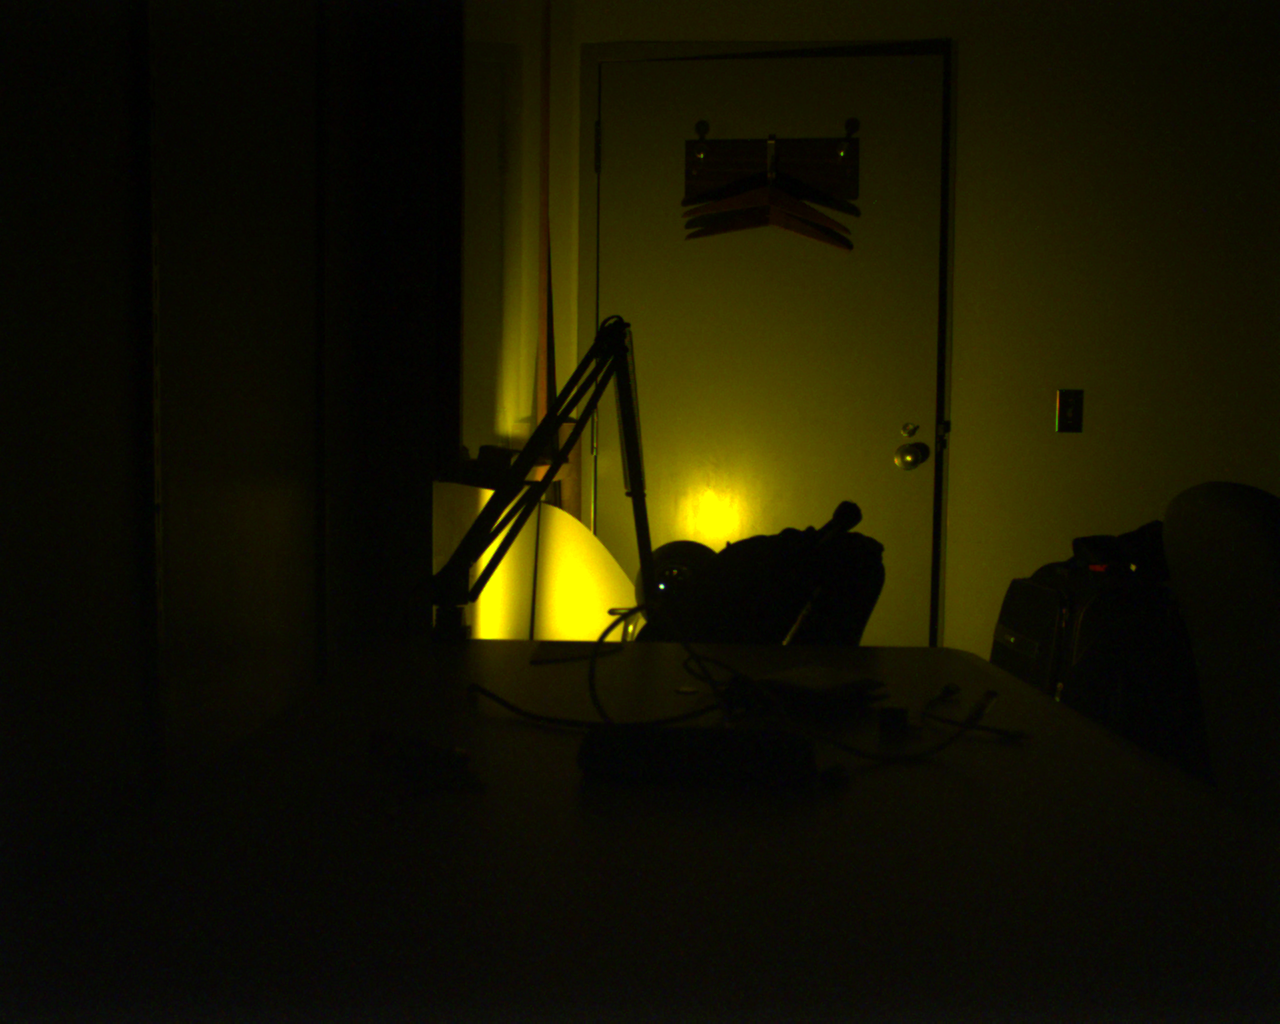
\includegraphics[width=\textwidth]{ui_img_33_ms_000.png}
			\caption{UI 33 ms exposure, minimum gain}
			\label{ui_img_33_ms_000}
		\end{subfigure}		
		\hfill
		\begin{subfigure}{0.3\textwidth}
			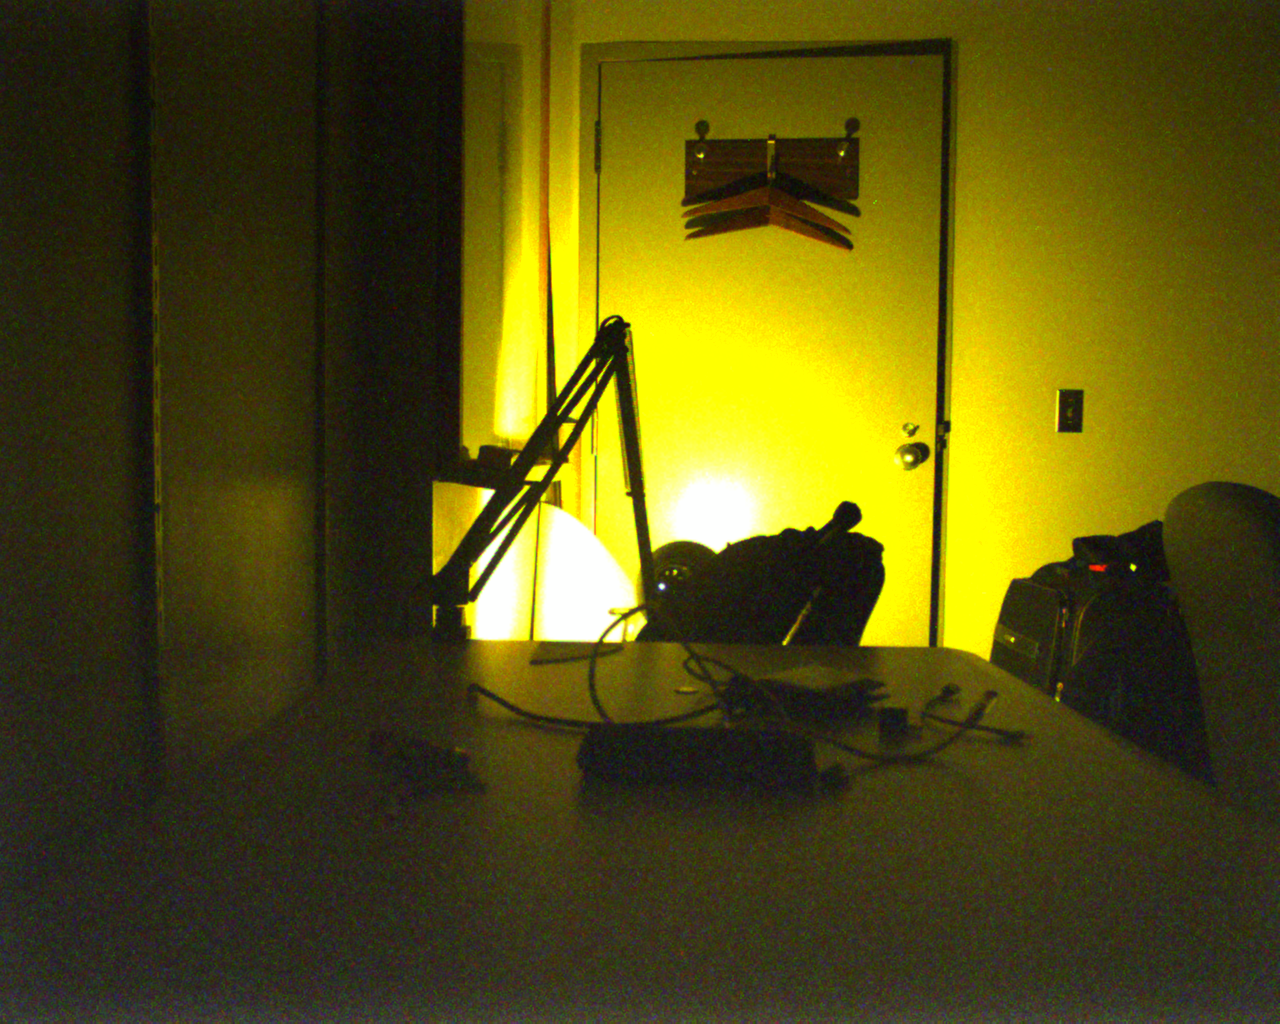
\includegraphics[width=\textwidth]{ui_img_33_ms_100.png}
			\caption{UI 33 ms exposure, maximum gain}
			\label{ui_img_33_ms_100}		
		\end{subfigure}
		\hfill
		\begin{subfigure}{0.3\textwidth}
			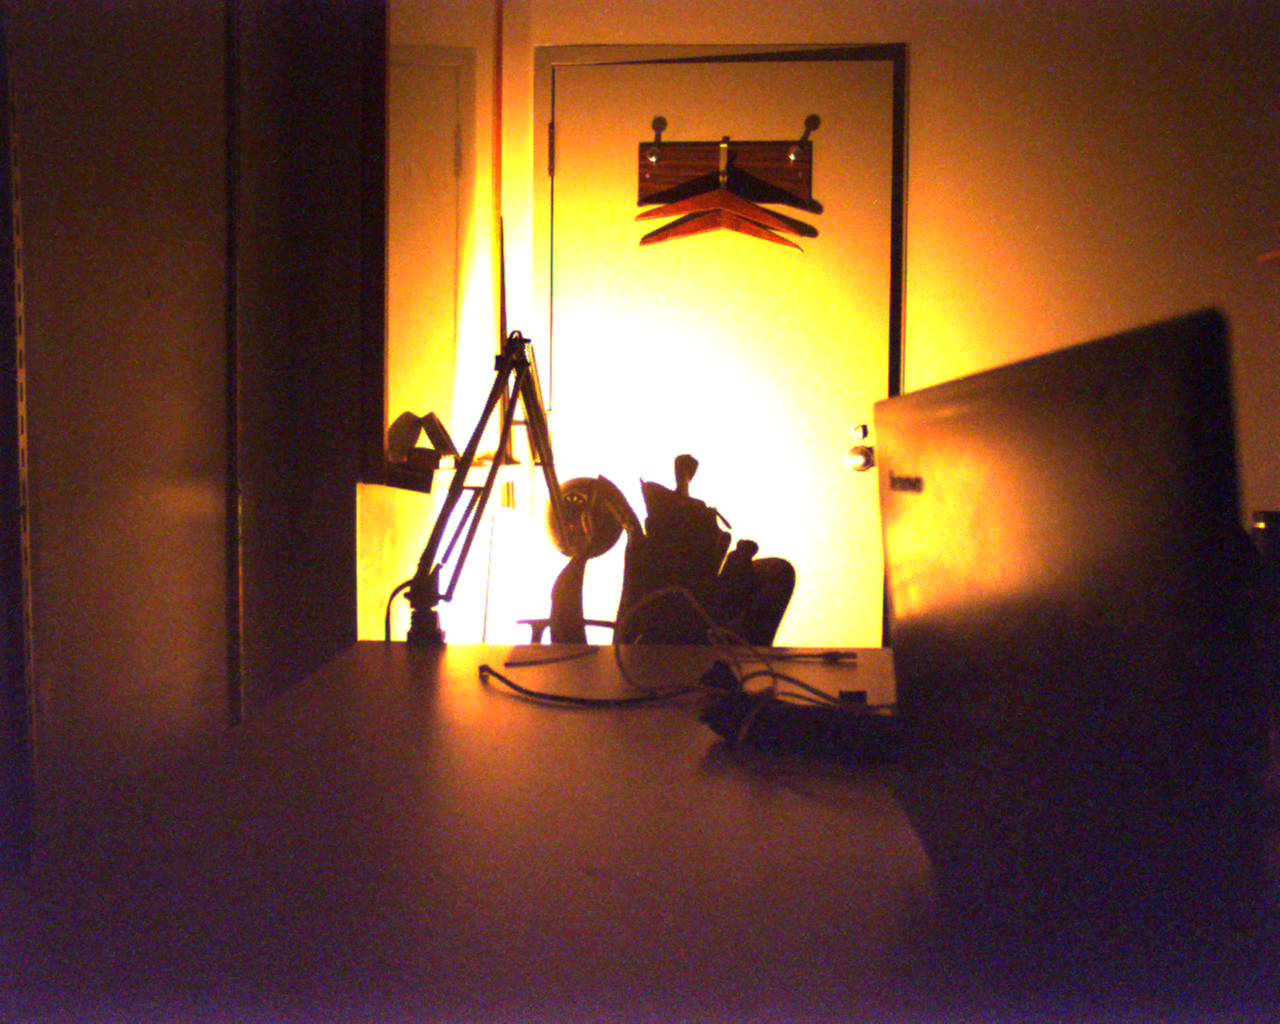
\includegraphics[width=\textwidth]{auto_ueye_2.png}
			\caption{UI automatic exposure, automatic gain}
			\label{auto_ueye_2}
		\end{subfigure}		
		\caption[RGB camera image quality comparison]{Comparison of image quality from UI-3241LE-C-HQ and RealSense D435 RGB cameras across a variety of gain values. Automatic exposure was limited to 33 ms due to a specified framerate of 30 fps for both cameras.}
		\label{camera_comparison}
	\end{figure}

	With manual gain enabled on both cameras, the images from the RealSense RGB camera are less bright, but exhibit significantly less noise than the images from the UI camera. Additionally, the UI camera's image at maximum gain \ref{ui_img_33_ms_100} saturated in the center, while the RealSense image did not, suggesting a lower dynamic range on the UI camera. When autoexposure was enabled on both cameras (\ref{auto_realsense_2}, \ref{auto_ueye_2}), the RealSense exhibited comparable noise to the UI camera, but produced an image with colors more accurate to the actual scene.
	
	When comparing synchronization ability, it appeared at first glance that both cameras supported external frame triggering, which allows frame capture to be driven by an external clock. This feature had previously been validated on the UI cameras in other lab projects. However, upon closer inspection it appeared that the external trigger for the RealSense module only applied to the depth module, and use of the external trigger would remove the synchronization between the RGB and depth modules on the RealSense camera. Similarly, when comparing shutter types, it appeared at first glance that both cameras had global shutters. This has also been previously validated on the UI cameras in other lab projects. However, further investigation revealed that the RealSense had a global shutter only for the 2 IR cameras used to compute depth, with the RGB camera instead having a rolling shutter.
	
	After this experiment, we decided to choose the RealSense D435 module for the Mk. 0 payload. We believed that the increase in image quality would outweigh the lack of external triggering and RGB camera rolling shutter. Additionally, the RealSense contained a depth module which eliminated the need for the selection of a separate depth camera. The RealSense also beat the UI camera in other payload goals - its price was less than $\frac{1}{2}$ of the UI camera, had shorter lead times which would allow for more rapid development, and had an enclosure which would simplify keeping the payload environmentally robust compared to the bare UI camera board.
	
	It should be noted that after this experiment was performed, it was discovered that the RealSense firmware version used had a bug when setting manual gain which lowered the maximum possible gain value. The automatic gain feature did not have this bug, which could explain why the RealSense image with automatic gain in \ref{auto_realsense_2} appears significantly brighter.
	
	\item[Thermal Camera] Stuff goes here
	\item[Microphone] stuff here
	\item[Wifi / Bluetooth scanning] here
	\item[Gas Sensor] stuff here
		
\end{description}

\subsection{Miscellaneous}

\begin{enumerate}
	\item Computers (for both object detection and SLAM)
	\item Sensing (both for SLAM and object detection), as well as sensor placement 
	\item sensor synchronization (maybe not its own bullet?)
	\item power management / distribution (everything in the box should be powered by a single cable)
	\item connectors (internal and external) (including debugging)
	\item heat dissipation (more of a mechanical problem)
	\item mounting
\end{enumerate}